\chapter{RF Schematic Design}
    \section{Matching Networks}
        Các matching networks thông thường chỉ sử dụng các \textbf{linh kiện lưu trữ năng lượng} 
        thay vì tiêu tán năng lượng. Đặc điểm này xuất phát tự nhiên từ mục đích 
        của matching networks, cụ thể là cho phép truyền \textbf{công suất tối đa} từ nguồn đến tải. 
        Nếu matching networks chứa các thành phần tiêu tán năng lượng, nó sẽ tiêu thụ một phần công suất 
        mà chúng ta đang cố gắng cung cấp cho tải. Do đó, matching networks sử dụng \textbf{tụ điện} 
        và \textbf{cuộn cảm}, chứ không phải điện trở.\cite{allaboutcircuits_matchingNetworks}\par

        Rất khó để thiết kế một matching networks băng thông rộng, do matching networks bao gồm các tụ điện và cuộn cảm.
        Bởi vì trở kháng của cuộn cảm và tụ điện phụ thuộc vào tần số, do đó việc thay đổi tần số của tín hiệu đi qua matching networks 
        có thể khiến nó kém hiệu quả hơn.\par

        \begin{figure}[h]
            \centering
            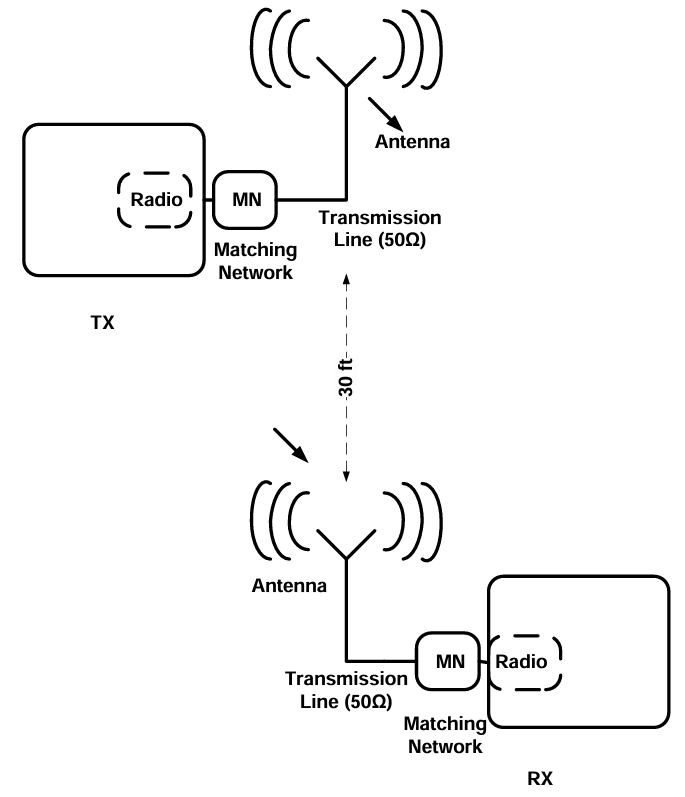
\includegraphics[width=0.45\textwidth]{figures/wireless_system.png}
            \caption{Typical Short-Range Wireless System}
            \label{fig:wireless_system}
        \end{figure}
        \newpage

        Về cơ bản, antenna là một dây dẫn lộ ra ngoài không gian. Nếu một dây dẫn có một tỉ lệ nhất định,
        hoặc là bội số bước sóng của tín hiệu\footnote{Harmonic antenna operation}, dây dẫn đó sẽ trở thành một antenna.
        Đây là điều kiện \textit{cộng hưởng}, vì năng lượng điện cung cấp cho antenna được bức xạ vào không gian.\cite{Infineon2023_rflayout}
        \autoref{fig:dipole_antenna_basic}
        \begin{figure}[h]
            \centering
            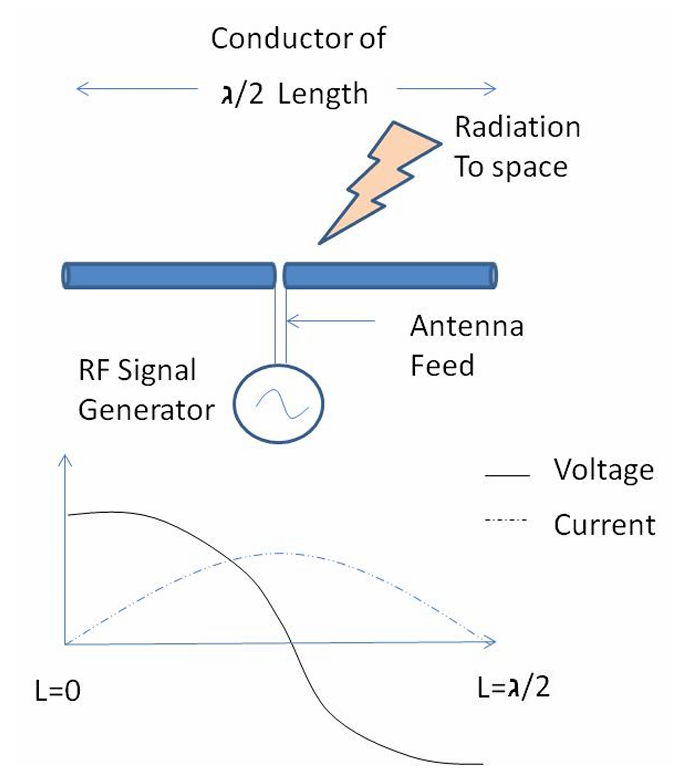
\includegraphics[width=0.5\textwidth]{figures/dipole_antenna_basic.png}
            \caption{Dipole Antenna Basic}
            \label{fig:dipole_antenna_basic}
        \end{figure}